\section{Motivation}
\label{sec:motivation}
\graphicspath{{_Intro/Figures/}}

The demand for wireless capacity to access the internet has greatly increased with rise in use of mobile computing devices including, laptops, tablets, and phones. We are increasingly using the internet to access articles, financial services, social networking, shopping, multimedia applications, gaming etc to name a few. There is ongoing research and increasing commercial activity in the field of smart spaces where everything from appliances, gadgets, power grid to home security are networked via cloud based services. These devices have been widely adopted and have become an integral part of our daily lives. The Cisco visual networking index (VNI) forecast \cite{cis14a} illustrated in \figurename{ \ref{fig:vnigraph}} predicts increase in networked traffic at a cumulative rate of 61$\%$ per year -- thus network traffic shall double every two years. 

With increase in use of mobile devices to access online services, wireless is increasingly the preferred method for internet access. This is currently being accomplished using the electromagnetic radiation within the radio frequency (RF) spectrum. The RF spectrum is a limited resource and the existing spectral allocations limit the ability to increase the system capacity thus making it ever so difficult to keep up with the wireless demand. In contrast to RF, light-based communication, and particularly the visible spectrum, is underutilized, unregulated and has the potential to be exploited to provide extra capacity to meet the demand for wireless communications especially for indoor spaces. 

\begin{figure}[!t]
	\centering
		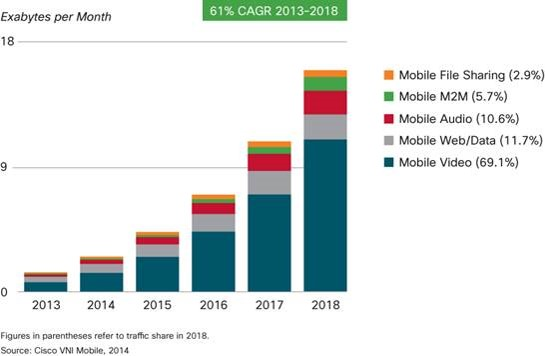
\includegraphics[width=5in]{vnigraph.jpg}
	\caption[Cisco VNI forecast]{Cisco VNI forecast \cite{cis14a}}
	\label{fig:vnigraph}
\end{figure}

Advances in solid state lighting has revolutionized the lighting industry. The realized energy and cost savings are leading the adoption of light-emitting-diode (LED) as the preferred source of illumination. \figurename{ \ref{fig:socketpenetration}} \cite{bar11a} predicts a worldwide socket penetration of at least 55$\%$ by year 2020. Lighting companies are now competing to replace all existing lighting fixtures with the new energy--efficient LED devices. Because lighting is well positioned to support human activities, it is also well positioned to serve as a highly localized wireless access vehicle by modulating the visible spectrum (380 nm -- 780 nm). This model is called the `dual use' of lighting and communication. In a practical implementation, overhead luminaires provide light and data downlink as an offload medium, being augmented by the availability of other media including RF as part of a heterogeneous network \cite{gan13a,rah15a}. 

\begin{figure}[!t]
	\centering
		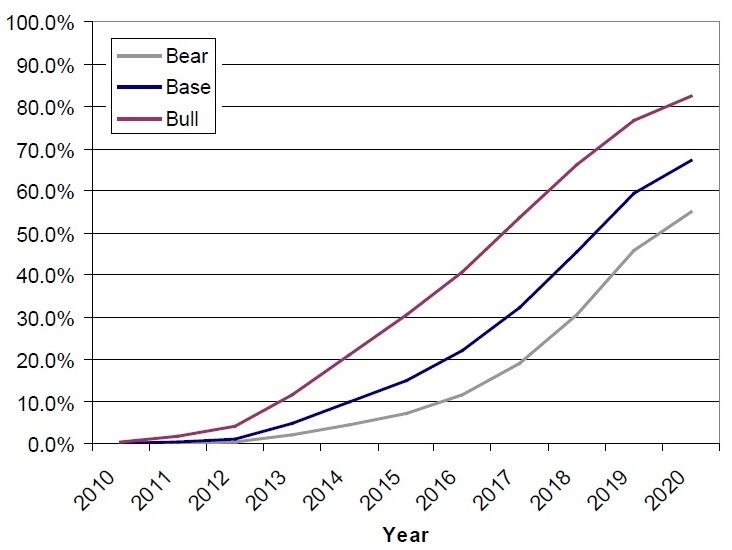
\includegraphics[width=5in]{socketpenetration.jpg}
	\caption[Total cumulative worldwide socket penetration]{Total cumulative worldwide socket penetration \cite{bar11a}}
	\label{fig:socketpenetration}
\end{figure}

The output luminous flux from an LED varies proportional to the current through the device. Information transmission can be achieved by modulating the current at a relatively high frequency ($>$ 200 Hz), generating a corresponding luminous flux, whose fluctuations are imperceptible to human eye. An optical receiver can sense this fluctuating illumination pattern and extract the transmitted information. This form of information transfer is known as intensity modulation / direct detection (IM/DD) and is widely used for optical wireless communication (OWC). Under this model, each light in an indoor space can be deployed as a wireless access point while providing illumination. Directionality of light along with high attenuation while propagating through walls provides an extra layer of security for information exchange with light in indoor spaces. Deploying multiple devices within the indoor space can enable spatial reuse over non-overlapping cones of illumination thus providing high bandwidth density.

A simple OWC link can be established by incorporating an LED as a transmitter and a photodiode (PD) as a receiver. The LED primarily services the function of providing illumination. At the same time, it can transmit information by rapidly changing its intensity. A typical illumination grade `white' LED uses a blue LED as the primary source of photons. The blue LED is encased in a phosphorescent encapsulant that emits yellow photons when excited by the blue photons. The blue and the yellow photons combine to generate white light for illumination. Different shades of white can be generated by changing the concentration of phosphorescent material. Phosphorescence is a slow process and limits the signal bandwidth that can be achieved in such a system to about 1 MHZ -- 2 MHz.

Different research groups have investigated optical signal bandwidth extension techniques. Techniques to improve achievable spectral efficiency of a single-input single-output (SISO) OWC system have also been well investigated. Spatial and wavelength based multiple-input multiple-output (MIMO) system proof of concepts have been reported in literature. Some of this research is summarized in the next section. The primary aim of the above enhancements was to demonstrate feasibility of optical spectrum to provide high speed wireless communication. Very little focus was given to given to achieve the primary function of a lighting fixture -- illumination. 

Incorporation of illumination targets while seamlessly providing wireless access is important for indoor OWC systems to be practically adopted. For OWC to be a viable candidate for mitigating `bottleneck' on wireless downlink, the achievable data rates per user need to be at least of the same order as those using RF. Thus it is important to improve the performance of optical modulation techniques and achievable spectral efficiencies using the optical spectrum. To that end, this dissertation investigates MIMO OWC systems under illumination targets and improves upon the state of the art by better utilizing the spatial and color dimensions. 


